%
% homotopie.tex
%
% (c) 2025 Prof Dr Andreas Müller, OST Ostschweizer Fachhochschule
%
\documentclass[tikz]{standalone}
\usepackage{times}
\usepackage{amsmath}
\usepackage{txfonts}
\usepackage[utf8]{inputenc}
\usepackage{graphics}
\usetikzlibrary{arrows,intersections,math}
\usepackage{ifthen}
\definecolor{darkred}{rgb}{0.8,0,0}
\definecolor{gelb}{rgb}{1,0.8,0}
\begin{document}

\newboolean{showgrid}
\setboolean{showgrid}{false}
\def\breite{3}
\def\hoehe{2}

\begin{tikzpicture}[>=latex,thick]

\clip (-9.03,-2.4) rectangle ++(12.6,4.8);

\begin{scope}
	% Povray Bild
	\node at (0,0) {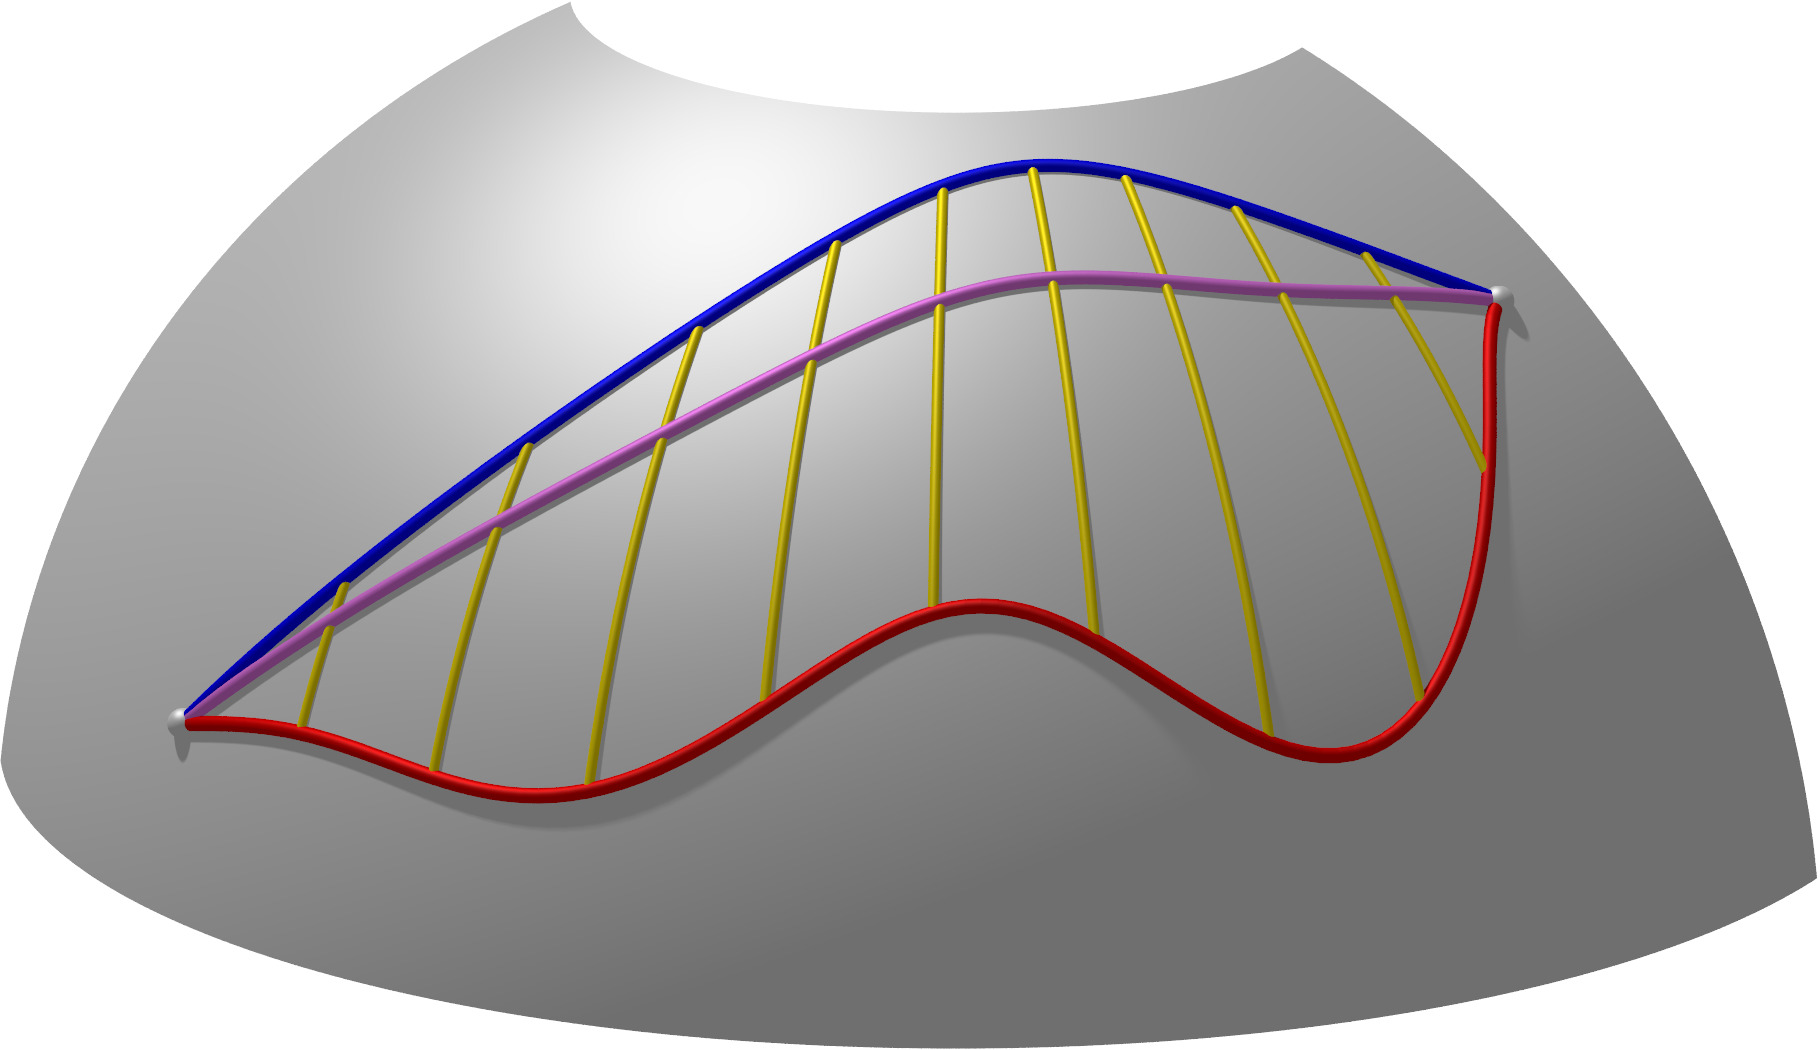
\includegraphics[width=7cm]{homotopie.jpg}};
	% Gitter
	\ifthenelse{\boolean{showgrid}}{
		\draw[step=0.1,line width=0.1pt]
			(-\breite,-\hoehe) grid (\breite, \hoehe);
		\draw[step=0.5,line width=0.4pt]
			(-\breite,-\hoehe) grid (\breite, \hoehe);
		\draw   (-\breite,-\hoehe) grid (\breite, \hoehe);
		\fill (0,0) circle[radius=0.05];
	}{}
	\node at (-1.4,1.6) {$M$};
	\node at (-2.75,-0.77) [left] {$A$};
	\node at (2.25,0.9) [right] {$B$};
\end{scope}

\begin{scope}[xshift=-8.7cm,yshift=-2cm]

	\fill[color=gray!20] (0,0) rectangle (4,4);
	\foreach \x in {0.1,0.2,...,0.9}{
		\draw[color=gelb] ({4*\x},0) -- ++(0,4);
	}
	\draw[->] (-0.05,0) -- (4.5,0) coordinate[label={below:$t$}];
	\draw[->] (0,-0.05) -- (0,4.3) coordinate[label={right:$s$}];
	\draw[color=darkred,line width=1.4pt] (0,0) -- ++(4,0);
	\draw[color=blue,line width=1.4pt] (0,4) -- ++(4,0);
	\draw[color=violet,line width=1.4pt] (0,2.4) -- ++(4,0);
	\node at (0,0) [below left] {$0$};
	\node at (4,0) [below] {$1$};
	\node at (0,4) [left] {$1$};

	\draw[->] (4.1,2) -- ++(1.2,0);
	\node at ({4.1+0.6},2) [above] {$H$};

	\draw[->,color=blue] (4.1,4) to[out=0,in=135] (7,2.4);
	\node[color=blue] at (5.5,3.9) [above] {$\gamma_1(t)=H(t,1)$};

	\draw[->,color=darkred] (4.1,0.1) -- (6.8,0.9);
	\node[color=darkred] at (4.8,0.5) [below right] {$\gamma_0(t)=H(t,0)$};


\end{scope}

\end{tikzpicture}

\end{document}

